
***
Holographic Characterization of Imperfect Colloidal Spheres
***

Holographic snapshots of colloidal spheres can be interpreted
with the Lorenz-Mie theory of light scattering to measure
an individual sphere's three-dimensional position,
size and refractive index \cite{lee07a}.
When applied to dielectric spheres with near-ideal sphericity
and smoothness, this technique yields nanometer-scale
precision for the position and radius 
\cite{lee07a,cheong10a,moyses13,krishnatreya14} 
and part-per-thousand precision for the refractive index 
\cite{lee07a,shpaisman12}.
Here, we demonstrate that this technique yields similarly precise 
and meaningful results for imperfect spheres, provided that their
deviation from sphericity is not too pronounced.


Such holograms then can be analyzed 
\cite{lee07a,cheong09,cheong10a,krishnatreya14a} with predictions of the
Lorenz-Mie theory of light scattering \cite{bohren83,mishchenko02} 
to estimate the particle's radius, $a_p$ and refractive index, $n_p$.
Specifically, we process a recorded image $I(\vec{r})$ by subtracting off the
camera's dark count, $I_d(\vec{r})$ and normalizing by a background image,
$I_0(\vec{r})$,
that is recorded with no particles in the field of view:
\begin{equation}
  \label{eq:normalized}
  b(\vec{r}) 
  =
  \frac{I(\vec{r}) - I_d(\vec{r})}{I_0(\vec{r}) - I_d(\vec{r})}.
\end{equation}
Assuming that gradients in the amplitude and phase of the illumination
are small over the scale of the particle, the normalized hologram of
a particle located at $\vec{r}_p$ relative to the center of the microscope's
focal plane may be modeled as \cite{lee07a,krishnatreya14}
\begin{equation}
  \label{eq:lorenzmie}
  b(\vec{r}) 
  =
  \abs{
    \hat{x} + e^{-i k z_p} \, \vec{f}_s(k(\vec{r} - \vec{r}_p))
  }^2,
\end{equation}
where $k = 2 \pi n_m / \lambda$ is the wave number of the light in a medium
of refractive index $n_m$, and where $\vec{f}_s(k\vec{r})$ 
describes how the particle scatters $\hat{x}$-polarized light.


If the particle may be modeled as
an ideal isotropic sphere, then $\vec{f}_s(k\vec{r})$ is
the Lorenz-Mie scattering function \cite{bohren83,mishchenko02},
which is parameterized by the particle's radius and refractive index.
Fitting Eq.~\eqref{eq:lorenzmie} to a measured hologram
therefore yields the particle's three-dimensional position $\vec{r}_p$,
its radius $a_p$ and its refractive index $n_p$.
Previous studies on model colloidal spheres have confirmed that
these fits converge reliably for micrometer-scale spheres, and yield
the radius with a precision better than 5 nanometers 
\cite{lee07a,moyses13,krishnatreya14}
and the refractive index to within 3 parts per thousand 
\cite{shpaisman12,moyses13}.
The data in Fig.~\ref{fig:singleparticle}(e) show results obtained for
a typical TPM sphere localized in an optical trap that was
projected through the microscope's objective lens using the
holographic optical trapping technique \cite{dufresne98,*grier03}.
The spread in values is comparable to the numerically
estimated uncertainty in the individual fits,
$a_p = \SI{0.790(3)}{\um}$ and $n_p = \num{1.445(1)}$,
suggesting both that
the imaging model is appropriate, and also that the signal-to-noise
ratio estimated by the median-absolute-deviation (MAD) metric
is reasonable.
This sphere's holographically measured radius is consistent with the 
mean value, \SI{0.76(6)}{\um}, obtained through SEM observations 
on the same batch of spheres.
The polymerized particles' refractive index is larger 
than that of monomeric TPM oil, \num{1.431} at the imaging wavelength.

The scattering function for an aspherical object, 
such as a dimpled sphere, depends on the object's detailed shape
and orientation \cite{mishchenko02}.
Analytical results are available for just a few special cases.
For more general cases, numerical methods are required, 
such as the discrete dipole approximation (DDA) \cite{draine94}. 
Even with highly optimized implementations \cite{yurkin11}, however,
such approaches are computationally intensive \cite{fung12,*perry12,*wang14using}.
If an object's departure from sphericity is small enough, and if the
influence of the non-ideality on the recorded hologram is sufficiently well
localized within the recorded image, Lorenz-Mie analysis
may still yield useful results for the particle's
size and refractive index without incurring this cost.

Figure~\ref{fig:singleparticle}(f) shows results obtained by fitting the
ideal-case model to holograms of an optically trapped dimpled sphere.
The radius estimated by straightforward 
Lorenz-Mie analysis of \num{60} such holograms
is \SI{0.821(6)}{\um}.
The corresponding estimate for the refractive index,
\num{1.448(1)} is remarkably similar to the value obtained for the
ideal spheres.
In both cases, the distribution of
values extracted from nonlinear least-squares 
fits to Eq.~\eqref{eq:lorenzmie} is consistent with single-fit error estimates.
This agreement suggests that the ideal model can yield quantitative
results for the characteristics of dimpled spheres, without incurring
the costs of more realistic modeling.

***
SVR
***

\section{Introduction}

Holograms of colloidal spheres obtained 
with holographic video microscopy
\cite{sheng06,lee07}
can be interpreted with predictions of the Lorenz-Mie theory 
of light scattering \cite{bohren83}
to track each particle in three dimensions, and to measure 
its size and refractive index \cite{lee07a}.
State-of-the-art implementations \cite{lee07a,bourquard13,seifi13,fung13}
can locate a sphere and resolve its
radius both to within a few nanometers, and 
can determine its refractive index to within a part per thousand
\cite{cheong09,shpaisman12,krishnatreya14}.
The cost of this powerful technique is the computational burden of
fitting each hologram pixel-by-pixel to theoretical predictions
\cite{lee07a,cheong10a}.
Here, we demonstrate that techniques of machine learning
can reduce the processing time by a factor of a thousand,
yielding real-time performance.
%The resulting real-time performance for single-particle
%characterization is fast enough for in-line process control,
%and creates new opportunities for soft-matter research.

Our approach to fast holographic characterization,
depicted schematically in Fig.~\ref{fig:method},
employs the support vector machine (SVM) algorithm
\cite{smola04} 
to compare experimental measurements with
pre-computed predictions of the Lorenz-Mie theory
\cite{bohren83,lee07a,krishnatreya14a}.
Whereas nonlinear fitting typically requires more than a second
on a \SI{1}{\giga flop} computer,
a trained SVM can estimate the size, refractive index or
axial position of a micrometer-scale sphere
in under a millisecond on the same hardware.

\begin{figure}
  \centering
  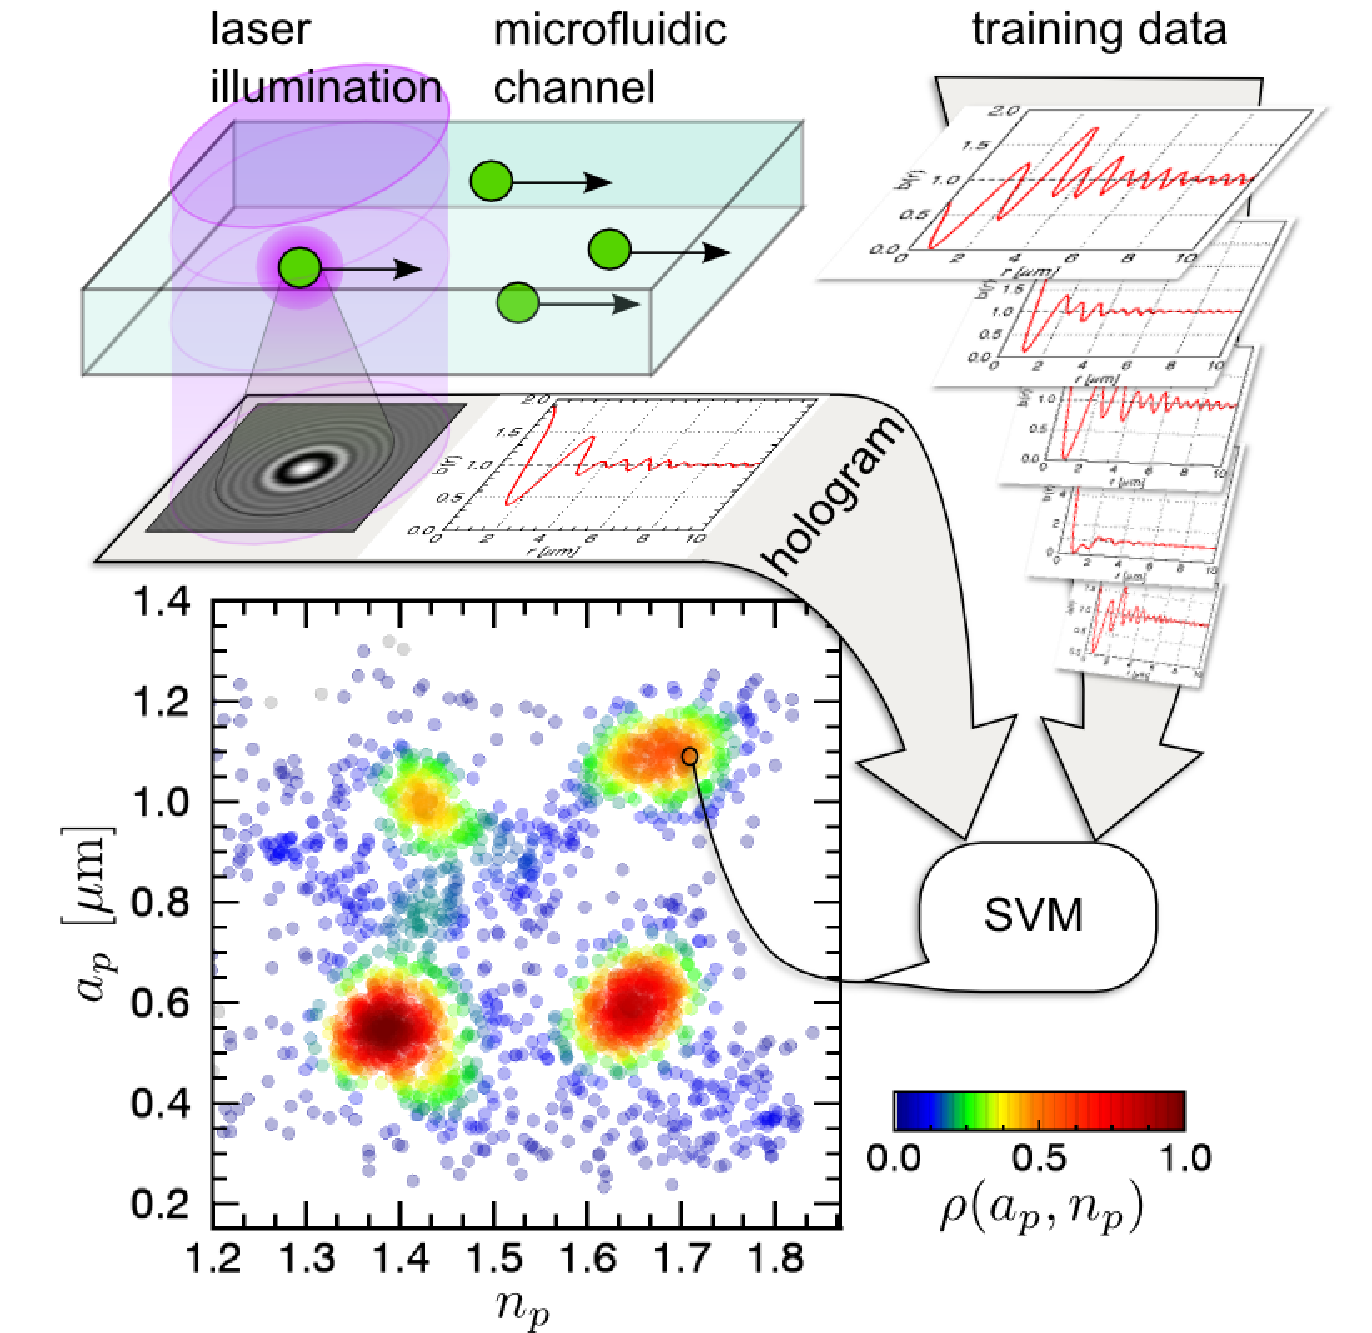
\includegraphics[width=0.7\textwidth]{svr_figure1}
  \caption{Colloidal characterization by holographic microscopy and
    machine learning.  Colloidal spheres flowing down a microfluidic
    sample scatter light from a collimated laser beam to form an
    in-line hologram.  Features in the beam are identified, and their
    radial profiles presented to support vector machines (SVMs)
    that compare them with a library of training data to estimate
    each spheres' radius $a_p$ and refractive index
    $n_p$.  The scatter plot shows results for 2,500 spheres
    drawn at random from a mixture of four different types of
    spheres.  Each point is colored by the local density of
    data points, $\rho(a_p,n_p)$.}
  \label{fig:method}
\end{figure}

\section{Fast Holographic Characterization with Machine Learning}

The in-line holographic microscope used for these studies
\cite{lee07,lee07a,krishnatreya14} 
illuminates the sample with a linearly polarized collimated
laser beam (Coherent Cube, \SI{20}{\mW})
at a vacuum wavelength of
$\lambda = \SI{447}{\nm}$.
The fluence of the \SI{3}{\mm}-diameter beam
is comparable to that of a conventional microscope illuminator.
Optical forces and light-induced heating therefore are negligible.
Light scattered by a sphere
propagates to the focal plane of a custom-built video microscope \cite{krishnatreya14}
where it interferes with the undiffracted portion of the original beam.
The microscope magnifies this interference pattern onto the detector of a greyscale
video camera (NEC TI 324AII), which records its intensity with a system
magnification of \SI{135}{\nm\per pixel}.
Each snapshot in the video stream constitutes a hologram of
the particles in the channel.

The electric field of the incident beam at position $\vec{r}$ in the focal plane
may be modeled as a plane wave with spatial dependence
\begin{equation}
  \label{eq:incidentfield}
  \vec{E}_0(\vec{r}) = u_0(\vec{r}) \, e^{i \varphi_0(\vec{r})} \, e^{i k z} \, \hat{x},
\end{equation}
where $k = 2 \pi n_m / \lambda$ is
the wavenumber in a medium of refractive index $n_m$, and
where $u_0(\vec{r})$ and $\varphi_0(\vec{r})$ account for small variations in the beam's
amplitude and phase profiles, respectively.

A particle located at $\vec{r}_p$ relative to the center of the focal
plane scatters the incident illumination,
$\vec{E}_0(\vec{r}_p)$, to the focal plane as
\begin{equation}
  \label{eq:scatteredfield}
  \vec{E}_s(\vec{r}) 
  = 
  E_0(\vec{r}_p) \, 
  \vec{f}_s\!\left( k (\vec{r} - \vec{r}_p) \vert a_p, n_p \right)),
\end{equation}
where $\vec{f}_s(k\vec{r} \vert a_p, n_p)$ is the Lorenz-Mie scattering function 
\cite{bohren83} that describes how a
sphere of radius $a_p$ and refractive index $n_p$ scatters an $\hat{x}$-polarized plane wave.
The measured
intensity then may be modeled as
\begin{equation}
  \label{eq:intensity}
  I(\vec{r}) 
  = 
  \abs{\vec{E}_0(\vec{r}) + \vec{E}_s(\vec{r})}^2.
\end{equation}
Normalizing the recorded hologram
by $I_0(\vec{r}) = \abs{\vec{E}_0(\vec{r})}^2 = u_0^2(\vec{r})$
suppresses spurious
structure in the illumination
and yields a functional form for the normalized hologram
\cite{lee07a,krishnatreya14},
\begin{equation}
  b(\vec{r}) 
  = \frac{I(\vec{r})}{I_0(\vec{r})}
  \approx
  \abs{
    \hat{x} + 
    e^{-i k z_p} \vec{f}_s(k(\vec{r} - \vec{r}_p)
    \vert a_p, n_p)}^2,
  \label{eq:theory}
\end{equation}
that can be calculated with standard software packages \cite{software}.

Previous implementations of Lorenz-Mie microscopy \cite{lee07a} 
fit Eq.~\eqref{eq:theory} to measured holograms using $a_p$, $n_p$
and $\vec{r}_p$ as adjustable parameters.
These fits are exquisitely sensitive to errors in the particle's
in-plane position, and so must be performed over the entire
two-dimensional intensity distribution \cite{lee07a}.
Here, we instead use Eq.~\eqref{eq:theory} to train
support vector machines, which then are able to estimate 
$a_p$, $n_p$ and $z_p$ from a hologram's one-dimensional
radial profile.
We obtain these profiles from measured holograms by averaging
around centers of rotational symmetry \cite{krishnatreya14a}
with single-pixel resolution, yielding 100-point data vectors.
The microscope's focal plane is adjusted so that the interference
fringes in a typical sphere's hologram extend to roughly this scale.
Averaging over angles to obtain a radial profile reduces the
dimensionality of the analysis problem and accounts in
part for our method's computational efficiency.

Our SVMs are 
implemented with {\tt scikit-learn}, an open-source
machine learning software package \cite{pedregosa11} that
builds upon the {\tt libsvm} library of Support Vector Machine algorithms
\cite{chang01,chang02}.
Each SVM computes one output parameter from an input vector
consisting of a radial profile, $b(r)$, that has been digitized
into 100 single-pixel bins.
Characterizing and tracking a colloidal particle therefore requires
three SVMs, one for each of $a_p$, $n_p$ and $z_p$.
Figure~\ref{fig:method} schematically represents this process
for estimating $a_p$ and $n_p$.



***
Feature-Finding
***


Holographic particle characterization \cite{lee07a} uses 
quantitative analysis of holographic video microscopy images to 
measure the size, shape, and composition of individual colloidal
particles, in addition to their three-dimensional positions.
When applied to a stream of dispersed particles, holographic
characterization measurements provide insights into the
joint distribution of particle size and composition
that cannot be obtained in any other way.
This technique has been demonstrated on both homogeneous
and heterogeneous \cite{yevick14,philips17}
dispersions of colloidal spheres, and has been extended to work for 
colloidal clusters \cite{perry12,fung12,fung13}, and aggregates 
\cite{wang16,wang16a}, as well as colloidal rods \cite{cheong10} 
and other aspherical particles \cite{wang14using,hannel15}.
Applications include
monitoring protein aggregation in biopharmaceuticals \cite{wang16},
detecting agglomeration in semiconductor polishing slurries
\cite{cheong17}, 
gauging the progress of colloidal synthesis reactions \cite{wang15,wang15a},
performing microrheology \cite{cheong08}, 
microrefractometry \cite{shpaisman12}, 
and microporosimetry \cite{cheong11} measurements,
assessing the quality of dairy products \cite{cheong09a},
and monitoring contaminants 
in wastewater \cite{philips17}.

The critical first step in holographic particle characterization
is to detect features of interest within a recorded video frame,
and to localize them well enough to enable subsequent 
analysis  \cite{crocker96,cheong09,yevick14,krishnatreya14a}.
False positive and negative detections clearly are undesirable.
Poor localization slows downstream analysis
\cite{yevick14,krishnatreya14a} and can prevent fitting algorithms 
from converging to reasonable results.
Here, we demonstrate that machine-learning algorithms can meet the
need for reliable feature detection and precise object localization in
holographic video microscopy.
This complements the previously reported \cite{yevick14}
use of machine-learning regression to estimate
characteristics such as particle size from holographic
features that already have been detected, localized
and isolated by other means.
With appropriate training, machine-learning algorithms
surpass standard image-analysis
techniques in their ability to cope with common image defects
such as overlapping features.
They also operate significantly faster, thereby enabling
applications that benefit from real-time performance on low-cost
hardware.

\begin{figure}[b!]
  \centering
  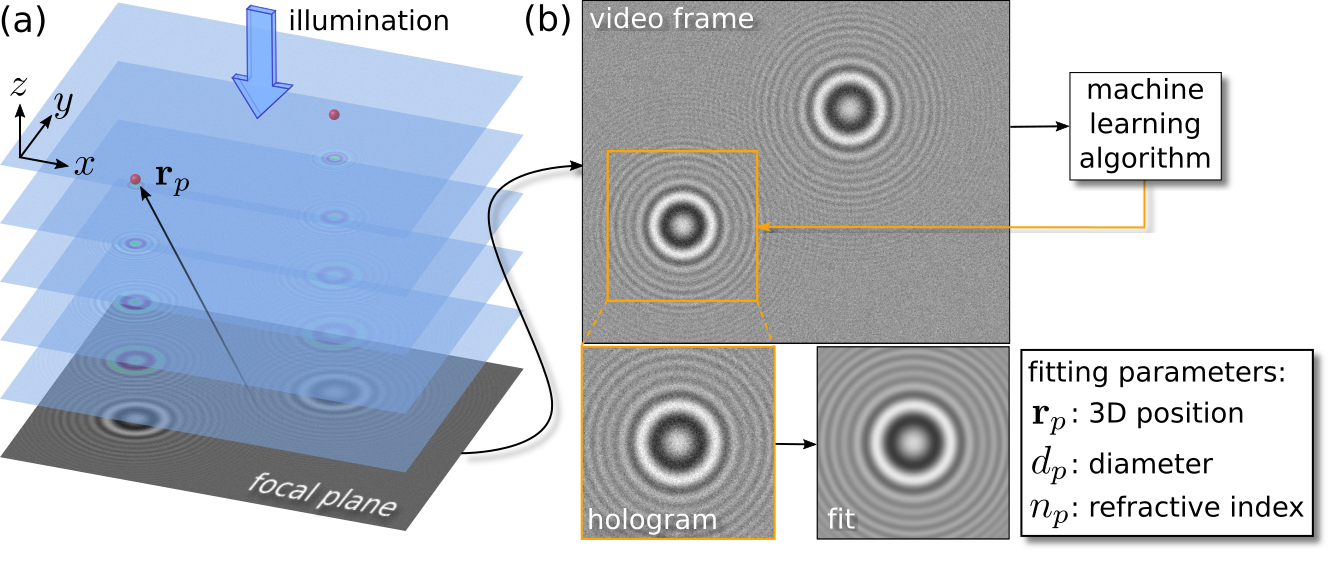
\includegraphics[width=0.9\textwidth]{cascade_01}	
  \caption{Overview of holographic particle characterization. (a) Plane-wave 
  illumination is scattered by colloidal particles (red spheres). The 
  field scattered by a particle at $\vec{r}_p$ interferes with the plane wave
  to produce a hologram in the focal
  plane of a microscope.
  (b) Features in a digitally recorded hologram are
  detected with a machine-learning algorithm before being
  analyzed with light-scattering 
  theory to estimate the particles' physical properties.}
  \label{fig:characterization}
\end{figure}

\section{Detecting and Localizing Holographic Features}

Figure~\ref{fig:characterization} illustrates the challenge of
recognizing features in holograms.
Light scattered by a particle 
spreads as it propagates to the focal plane of a conventional
microscope.
There, it interferes with the remainder of the illuminating beam
to create a pattern of concentric interference fringes.
The microscope magnifies this interference pattern and
projects it onto
the detector of a video camera.
The intensity variations
associated with a single colloidal particle
typically span many pixels in a recorded image
and display rich internal structure.
Their scale and complexity render such features difficult to
recognize by conventional
particle-tracking techniques.
  
